\documentclass[10pt,a4paper]{report}
\usepackage{graphicx, tabularx}
\usepackage{amsthm, amsfonts, amsmath, amssymb}
\usepackage{mathtools}
\usepackage{sectsty}
\usepackage[inline]{enumitem}
\usepackage{csquotes}
\usepackage{listings}
\usepackage{xcolor}
\usepackage[hidelinks]{hyperref}
\usepackage{cleveref}
\usepackage[english]{babel}
\usepackage{biblatex}
\usepackage{libertinus}

\theoremstyle{plain}
\newtheorem{theorem}{Theorem}
\newtheorem{lemma}{Lemma}

\theoremstyle{definition}
\newtheorem{definition}{Definition}
\newtheorem{example}{Example}

\theoremstyle{remark}
\newtheorem*{note}{Note}
\newtheorem*{remark}{Remark}

\addbibresource{bibliography.bib}

\allowdisplaybreaks
\setcounter{tocdepth}{1}
\chapternumberfont{\LARGE}
\chaptertitlefont{\huge}

\title{Extending Axiom Weakening for Automated Repair of Ontologies in Expressive Description Logics}
\author{Roland Bernard}
\date{July 2023}

\makeatletter
\def\maketitle{
    \begin{tabular}{ll}
        \multicolumn{2}{r}{
\includegraphics[width=0.5\linewidth]{resources/unibz-logo.png}} \\
        \vspace*{40mm} \\
        \multicolumn{2}{l}{\raggedright Bachelor Thesis} \\
        \vspace*{1mm} \\
        \multicolumn{2}{p{\linewidth}}{\raggedright \huge \bf \@title} \\
        \vspace*{30mm} \\
        Candidate   & \@author \\
        \vspace*{5mm} \\
        Supervisors & Oliver Kutz \\
                    & Nicolas Troquard \\
        \vspace*{20mm} \\
        \multicolumn{2}{p{\linewidth}}{\@date}
    \end{tabular}
}

\begin{document}

\maketitle

\begin{abstract}
    The field of ontology engineering plays a crucial role in knowledge representation and has gained significant attention in recent years in many domains such as medicine, finance, and education. The introduction of the W3C recommended Web Ontology Language has further enabled use cases for ontology engineering in the context of the semantic web. With the growing size and complexity of these ontologies, however, ontologies become more susceptible to bugs, and it becomes harder to debug these defects. While debugging in software engineering has received much attention, tooling support for debugging ontologies remains limited. Moreover, in the context of the semantic web, automatic approaches to debugging ontologies are required for the combination of knowledge derived from independent sources. Axiom weakening has been proposed as a solution for fine-grained repair to inconsistent ontologies. This thesis presents an extension to the axiom weakening operator, in the $\mathcal{SROIQ}$ description logic, to cover a wider range of axiom types, including role inclusion axioms and role assertions. I show that the presented weakening operator retains desirable properties satisfied by previous approaches. The presented automated repair approach is experimentally evaluated against other repair approaches on a number of inconsistent ontologies. The paper compares the amount of information that the repair is able to retain relative to other repairs based on the inferred concept hierarchy. Further, the implementation of the presented axiom weakening operator in the popular ontology editor, Protégé, is discussed. The efficacy of integrating axiom weakening in the manual debugging process is demonstrated for inconsistent ontologies and unintended consequences in general.

\end{abstract}

\tableofcontents

\begingroup
\renewcommand{\abstractname}{Acknowledgements}
\begin{abstract}
    Thanks Mami and Tati!

\end{abstract}
\endgroup

\chapter{Introduction} \label{introduction}


The field of ontologies plays a crucial role in knowledge representation and has gained significant attention in recent years in many domains, such as in biology and medicine. The introduction of the Web Ontology Language as a World Wide Web Consortium (W3C) recommendation has further grown the ecosystem and enabled use cases for ontology engineering in the context of the semantic web.

Ontologies provide a structured and formalized way to represent knowledge about particular domains and facilitate automatic reasoning and knowledge sharing. Nevertheless, the development and maintenance of ontologies is not without challenges. With the growing size and complexity of these ontologies, they become more susceptible to bugs, and it becomes harder to debug these defects. Furthermore, in the context of the semantic web, automatic approaches to correcting ontologies are needed for the combination of conflicting knowledge derived from independent sources.

The \SROIQ Description Logic is a very expressive variant of the Description Logics family, which can serve as the logical basis for representing knowledge in ontologies. It is also the foundation for the Web Ontology Language, a standardized language for representing ontologies on the web, enabling the creation of machine-readable ontologies. In both of these systems, ontologies are sets of axioms, and each axiom is a statement encoding some knowledge about the domain. \SROIQ extends upon basic description logics like \ALC with additional features such as complex role hierarchies, role disjointness axioms, and transitive roles. This expressive power allows for modelling complex domains with rich relationships and constraints. This expressivity, however, comes at the cost of requiring some global restrictions that must be followed in order to ensure the decidability of the logic.

Many approaches to repairing inconsistent ontologies amount to identifying problematic axioms and then removing them (e.g., ~\cite{schlobach2003non,kalyanpur2005debugging,kalyanpur2006repairing,BaPS07}). Whilst this approach is obviously sufficient to guarantee that the obtained ontology is consistent, it tends to lead to information loss as a secondary effect, as outlined in detail in related works \cite{troquard2018repairing,confalonieri2020towards}. 
Axiom weakening has been proposed as a solution for fine-grained repair to inconsistent ontologies. In these approaches, the information loss is reduced by weakening the inferential power of an axiom rather than by deleting it entirely \cite{du2014practical,AMAI-2018,baader2018making,troquard2018repairing,confalonieri2020towards}. 
%
In \cite{troquard2018repairing}, axiom weakening using refinement operators has been described for \ALC and experimentally evaluated, showing that axiom weakening is able to retain more information than deletion. In \cite{confalonieri2020towards}, axiom weakening is extended to include many aspects of \SROIQ, notably omitting, however, the weakening of RBox axioms.

This thesis aims to explore the topic of ontology repair, specifically focusing on axiom weakening in the context of the \SROIQ Description Logic and the Web Ontology Language. It extends upon the previous work on axiom weakening in description logics by extending the underlying basic principles to the logic \SROIQ, including also the possibility of weakening role inclusion axioms and disjoint role axioms. The thesis examines the challenges and difficulties that arise when applying axiom weakening to these more expressive description logics, and covers a number of scenarios where weakening can affect regularity of \SROIQ RBoxes. Further, a framework where these problems can be prevented is proposed.

The implementation of the proposed algorithms will be discussed. Next to a prototype implementation used primarily for running the experimental evaluation, a plugin for the popular ontology editor, Protégé, has been realized. The thesis presents some details of the implementation process and discusses the integration of axiom weakening functionalities into the Protégé tool.

Additionally, by implementing the proposed refinement and weakening operators it becomes possible to perform experimental evaluation, also on ontologies using the more expressive features of \SROIQ. The quality of repairs achieved through axiom weakening is assessed, and the results reaffirm the findings of \cite{troquard2018repairing} for the case of \SROIQ, namely that weakening may significantly outperform deletion. Additionally, the thesis explores the impact of caching in cover computations and evaluates the performance in terms of reasoner calls and execution time.

Finally, the thesis concludes with a summary of the findings, their implications, and possible directions for future research. By addressing some of the challenges related to axiom weakening in the \SROIQ Description Logic, this research aims to contribute to the field of ontology engineering and inspire further research into axiom weakening and ontology repair.


\chapter{Background and Related Work} \label{background}

\section{Ontology Bugs} \label{ontology-bugs}


As software systems evolve, it becomes harder to avoid the introduction of bugs. Similarly, in ontology engineering, bugs can be introduced into an ontology. With increased size and complexity of a system, it becomes harder to debug these defects, both for software systems and ontologies.

\subsection{Categories of Bugs} \label{categories-of-bugs}

Defects, in both software systems and ontologies, can be due to a number of different reasons. In \cite{kalyanpur2005debugging} the authors identify three broad categories of defects that can be present in an ontology: \emph{syntactic defects}, \emph{semantic defects,} and \emph{modelling defects}.

\subsubsection{Syntactic Defects} \label{syntactic-defects}

Syntactic defects in an ontology can be caused by a statement that does not conform to the grammar of the employed logic. Similarly, for software systems, these defects may be the result of programs that are not consistent with the grammar of the chosen programming language. These sorts of syntactic defects are easy to locate and correct. In general, tool support for these kinds of defects is able to pinpoint the location of the defect and give an explanation to the user.

\begin{example}
% TODO
\end{example}

There may however be some additional restrictions on what constitutes a valid ontology or program that is not based solely on the grammatical rules. For ontologies, these might be for example the restrictions placed upon the form of the graph for a specific OWL profile. For programming languages, a similar restriction to this may be the requirement for definition before use or the presence of a type system\footnote{When viewed from a different perspective, a type error can also be seen as the unsatisfiability of (or ambiguity in) the type assertions. In this way, it is related to an inconsistency in the context of ontologies in the case of unsatisfiability (or missing inferences in the case of ambiguity).}. These restrictions reduce the space of valid programs. Restrictions of this kind can often be much easier to violate and harder to debug than the first kind of syntactic defects that is a violation of the grammar.

\begin{example}
% TODO
\end{example}

\subsubsection{Semantic Defects} \label{semantic-defects}

For ontologies, semantic defects, as defined in \cite{kalyanpur2005debugging}  are those which can be discovered by a reasoner given an ontology free of syntactic defects. This includes for example the inconsistency of the ontology, or the unsatisfiability of a concept. The presence of such defects is generally not hard to identify, given the availability of a reasoner for the logic of the ontology. It is, however, often not trivial to understand the underlying source of the defect.

\begin{example}
% TODO
\end{example}

A close analogy to these kinds of defects from the perspective of a software system is the raising of an error during the execution. An error is an indication of a defect in the software, and depending on tooling support they may be more or less difficult to understand and rectify.

\subsubsection{Modelling Defects} \label{modelling-defects}

Modelling defects are those defects that are not syntactically or semantically invalid. The presence of unintended inferences in an ontology is one such defect. These defects can also be of more stylistic nature. Redundancy or unused parts of the ontology may be considered as defects, since they do not add any knowledge to the ontology.

For software systems, modelling defects are bugs that do not cause any errors, but which produce undesired behaviour. An example for such a defect could be that the result of a calculation is wrong, or that the software includes security vulnerabilities. For software systems, there might be other non-functional requirements, that if not met constitute defects in the software. These may for example be unsatisfactory performance or unmaintainable code organization.

These kinds of defects can in general not be detected automatically by tools. They require careful attention and domain specific knowledge to be revealed and corrected. In some scenarios, testing may be used to uncover and prevent against some modelling defects, by expressing more explicitly the modellers/programmers intend. This can be done both for software systems and for ontologies.

\subsection{Causes of Bugs} \label{causes-of-bugs}

% TODO


\section{Ontologies in Description Logics} \label{ontologies-in-dl}


While ontologies can be represented using a number of different formalisms, for the use in automated reasoning a trade-off must be made between expressivity and practicality. For example, first-order logic (FOL) is more expressive than propositional logic, but this added expressivity comes at the cost of decidability. In addition to decidability, scalability must also be considered in the choice and design of the used representation of the knowledge.

\emph{Description logics} (DL) are often used for building ontologies. They encompass a family of related knowledge representation languages and are often fragments of FOL\footnote{While description logics are fragments of FOL in the sense that for every knowledge base in a given description logic, there exists a FOL theory that has the same models, the syntax used by description logics is different from the syntax used in FOL, and as such a DL axiom is not a valid FOL sentence.} with equality, as is the case with the description logics $\mathcal{SROIQ}$ which is the main focus of this work. DLs are almost always designed to be decidable, and generally offer a favourable trade-off between expressivity and complexity of reasoning tasks. Different description logics have been developed for different applications, that feature varying levels of expressivity.

Description logics are also the basis of the \emph{Web Ontology Language} (OWL) \cite{hitzler2009owl_primer,motik2009owl_spec}, which is a World Wide Web Consortium (W3C) recommendation and is extensively used as part of the semantic web. While the OWL 2 language is based on $\mathcal{SROIQ}$, OWL 2 also defines three so-called profiles that are fragments of the full OWL 2 language that trade-off expressive power for more efficient reasoning \cite{motik2009owl_profiles,motik2009owl_spec}. The OWL 2 DL profile, which is the most expressive of the profiles that is still decidable\footnote{The most expressive profile, OWL 2 Full, is not decidable.}, is based on $\mathcal{SROIQ}$.

The following sections will introduce the description logic $\mathcal{SROIQ}$ and the OWL 2 language. The relation between the two will also be discussed. The description is based on the one presented in \cite{rudolph2011foundations}.

\subsection{The \texorpdfstring{$\mathcal{SROIQ}$}{SROIQ} Description Logic} \label{sroiq-def}

\subsection{\texorpdfstring{$\mathcal{SROIQ}$}{SROIQ} Syntax} \label{sroiq-syntax}

\input{sections/2.2.1.1.sroiq-syn.tex}

\subsection{\texorpdfstring{$\mathcal{SROIQ}$}{SROIQ} Semantics} \label{sroiq-semantics}

\input{sections/2.2.1.2.sroiq-sem.tex}



\subsection{The Web Ontology Language} \label{owl-def}


Description logics are also the basis of the \emph{Web Ontology Language} (OWL) \cite{hitzler2009owl_primer,motik2009owl_spec}, which is a World Wide Web Consortium (W3C) recommendation and is extensively used as part of the semantic web. While the OWL 2 DL language is based on $\mathcal{SROIQ}$, OWL 2 also defines three so-called profiles that are fragments of the full OWL 2 language that trade-off expressive power for more efficient reasoning \cite{motik2009owl_profiles,motik2009owl_spec}. The OWL 2 DL profile, which is the most expressive of the profiles that is still decidable\footnote{The most expressive profile, OWL 2 Full, is not decidable.}, is based on $\mathcal{SROIQ}$.





\section{Repairing Ontologies} \label{ontology-repair}


As established in \cref{ontology-bugs}, maintaining the consistency and correctness of ontologies can be a difficult task. Ontology repair is the process of automatically correcting these inconsistencies or errors in ontologies. Several approaches have been proposed for ontology repair.  This section will explore some of these approaches and their underlying principles.

\subsection{Basic Definitions} \label{basic-definitions}

We define a repair as proposed in \cite{baader2018making}. It is assumed, as is the case for most description logics, that there exists a monotone consequence operator $\vDash$ such that for any two ontologies $\mathcal{O}_1 \subseteq \mathcal{O}_2$ and axiom $\alpha$, $\mathcal{O}_1 \vDash \alpha$ implies $\mathcal{O}_2 \vDash \alpha$. Additionally, $\mathrm{Con}(\mathcal{O})$ shall contain all consequences of $\mathcal{O}$, that is $\mathrm{Con}(\mathcal{O}) = \{ \alpha \mid \mathcal{O} \vDash \alpha \}$. We split the ontology further into two disjoint sets $\mathcal{O} = \mathcal{O}_s \cup \mathcal{O}_r$ of \emph{static axioms} $\mathcal{O}_s$ and \emph{refutable axioms} $\mathcal{O}_r$. Static axioms are assumed to be correct and may not be touched by the repair procedure, while refutable axioms are possibly be erroneous. This separation is useful for example if the static part of the ontology is hand-crafted, while the refutable part is automatically generated. Similarly, it is applicable in case multiple ontologies are combined, and some sources are seen as less trustworthy than others.

\begin{definition}
Given an ontology $\mathcal{O} = \mathcal{O}_s \cup \mathcal{O}_r$ and an unintended consequence $\mathcal{O} \vDash \alpha$, $\mathcal{O}_s \not\vDash \alpha$, the ontology $\mathcal{O}_s \subseteq \mathcal{O}'$ is a \emph{repair} of $\mathcal{O}$ with respect to $\alpha$ if $\mathrm{Con}(\mathcal{O}') \subseteq \mathrm{Con}(\mathcal{O}) \setminus \{\alpha\}.$ A repair $\mathcal{O}'$ is an \emph{optimal repair} of $\mathcal{O}$ with respect to $\alpha$ if there exists no other repair $\mathcal{O}_s \subseteq \mathcal{O}''$ such that $\mathrm{Con}(\mathcal{O}') \subset \mathrm{Con}(\mathcal{O}'') \subseteq \mathrm{Con}(\mathcal{O}) \setminus \{\alpha\}$.
\end{definition}

Given that $\mathcal{O}_s \not\vDash \alpha$, a repair is guaranteed to exist, since $\mathcal{O}_s$ is one such repair. In contrast, generally an optimal repair does not need to exist.

\begin{example}
%TODO
\end{example}

It should be noted also that there exists an infinite number of possible repairs, as adding tautologies to a repair will yield another valid repair. In the case that we are interested in making an inconsistent ontology consistent, we can use as $\alpha$ an unsatisfiable axiom, e.g., $\top \sqsubseteq \bot$. Since all axioms, including unsatisfiable axioms, are entailed by inconsistent ontologies, a repair that does not entail $\alpha$ is consistent. Notice also that in this case where $\mathcal{O}$ is inconsistent, any consistent ontology that does not entail $\alpha$, even if completely unrelated to $\mathcal{O}$, will be a repair of $\mathcal{O}$.

In contrast, the classical approach to repair consists of locating and removing problematic axioms. As such, a classical repair is always a subset of the original ontology and the number of classical repairs for any pair $\mathcal{O}$ and $\alpha$ is necessarily finite.

\begin{definition}
Given an ontology $\mathcal{O} = \mathcal{O}_s \cup \mathcal{O}_r$ and an unintended consequence $\mathcal{O} \vDash \alpha$, $\mathcal{O}_s \not\vDash \alpha$, the ontology $\mathcal{O}_s \subseteq \mathcal{O}' \subseteq \mathcal{O}$ is a \emph{classical repair} of $\mathcal{O}$ with respect to $\alpha$ if $\mathrm{Con}(\mathcal{O}') \subseteq \mathrm{Con}(\mathcal{O}) \setminus \{\alpha\}.$ A classical repair $\mathcal{O}'$ is an \emph{optimal classical repair} of $\mathcal{O}$ with respect to $\alpha$ if there exists no other classical repair $\mathcal{O}_s \subseteq \mathcal{O}'' \subseteq \mathcal{O}$ such that $\mathrm{Con}(\mathcal{O}') \subset \mathrm{Con}(\mathcal{O}'') \subseteq \mathrm{Con}(\mathcal{O}) \setminus \{\alpha\}$.
\end{definition}

We can observe that every classical repair is in fact a valid repair. It follows that also a classical repair is guaranteed to exist. Unlike for the general case of optimal repairs, an optimal classical repair is always guaranteed to exist. This follows from the fact that the set of classical repairs is finite, and the $\subset$ relation is a strict partial order, so there can not be an infinite sequence of classical repairs $\mathcal{O}^{(1)}, \mathcal{O}^{(2)}, \dots$  such that $\mathrm{Con}(\mathcal{O}^{(i)}) \subset \mathrm{Con}(\mathcal{O}^{(i + 1)})$.

\subsection{Repair Approaches} \label{repair-approaches}

\subsubsection{Classical Repairs} \label{classical-repairs}

Generating a classical repair can be achieved in a number of equivalent ways. One way to compute an optimal classical repair is using justifications and hitting sets \cite{reiter1987theory}.

\begin{definition}
Given an ontology $\mathcal{O} = \mathcal{O}_s \cup \mathcal{O}_r$ and an axiom $\mathcal{O} \vDash \alpha$, $\mathcal{O}_s \not\vDash \alpha$, a \emph{justification} for $\alpha$ in $\mathcal{O}$ is a minimal subset $J \subseteq \mathcal{O}_r$ such that $J \cup \mathcal{O}_s \vDash \alpha$. Given the set of all justifications $J_1, \dots, J_n$ for $\alpha$ in $\mathcal{O}$, a \emph{hitting set} $H$ for these justifications is a set of axioms such that $H \cap J_i \not= \empty$ for $i = 1, \dots, n$. $H$ is a \emph{minimal hitting} set if it does not strictly contain another hitting set.
\end{definition}

\begin{example}
%TODO
\end{example}

Justifications are necessarily non-empty since $\mathcal{O}_s \not\vDash \alpha$, and therefore hitting sets and minimal hitting sets always exist. Given any minimal hitting set $H$ for the justification $J_1, \dots, J_n$ of $\alpha$ in $\mathcal{O}$, the ontology $\mathcal{O}' = \mathcal{O} \setminus H$ is an optimal classical repair of $\mathcal{O}$ with respect to $\alpha$.

This algorithm for computing optimal classical repairs requires the computation of all justifications, which can in general be very computationally intensive. Black-box approaches for computing justifications have been proposed \cite{kalyanpur2007finding,schlobach2003non,schlobach2007debugging} that compute justifications by repeatedly making calls to pre-existing highly-optimized reasoners. These may however, in the worst-case, need to make an exponential number of calls to the reasoner. Nevertheless, in practice they may often be fast enough, as for example the hitting set tree base algorithm presented in \cite{kalyanpur2007finding}, which conveniently can compute both all justifications and all hitting sets. There exist also glass-box approach to computing justifications \cite{kalyanpur2007finding}, that require only a single reasoning request to find justifications, but they also require specialized, generally less efficient, reasoners.

An alternative to computing all justification is to directly find a minimal correction subset $C$ of $\mathcal{O}_r$ such that $\mathcal{O} \setminus C \not\vDash \alpha$. Finding a single such set can be done efficiently using similar algorithms to the ones for finding single justifications. Algorithms for solving the minimal subsets over monotone predicate problem, such as the \textsc{QuickXplain} algorithm \cite{junker2004preferred} or a progression-based algorithm \cite{marques2013minimal} may be used. A subset of all such sets can be found efficiently using the \textsc{MergeXplain} algorithm \cite{shchekotykhin2015mergexplain}. Of course, computing all minimal correction subsets directly is also possible, using similar algorithms to the ones used for computing all justifications \cite{malouf2007maximal}.

\subsubsection{More Gentle Repairs} \label{more-gentle-repairs}

While the classical approach is sufficient to guarantee finding a repair of the ontology, it can lead to information loss. That is, the repaired ontology might be missing some consequences of the original ontology that were actually desirable.

\begin{example}
%TODO
\end{example}

Since ideally, one wants to retain as much information as possible, alternative methods for repairing ontologies have been proposed that are able to preserve more information than the classical approach.

One option is to first modify the original ontology and afterwards apply the classical repair approach. The intuition is that in the modified ontology the individual axioms contain less information, and therefore the removal of axioms can be more granular relative to the unmodified ontology. In \cite{horridge2008laconic} the authors propose a structural transformation, that replaces axioms with a set of weaker axioms that are semantically equivalent.

\begin{example}
%TODO
\end{example}

Another approach to repairing ontologies more gently that has been proposed in the literature is using \emph{axiom weakening} \cite{troquard2018repairing,confalonieri2020towards,confalonieri2022irresistible,baader2018making,lam2008fine}. Instead of removing axioms, they are replaced with weaker axioms. In \cite{lam2008fine} the authors show a method for pinpointing the causes for unsatisfiability a within axioms, and propose a way of weakening axioms guided by this information. The authors of \cite{baader2018making} show general theoretical results for repair using axiom weakening, and propose a concrete weakening relation for the $\mathcal{EL}$ description logics. They further show that the repair algorithm using the proposed axiom weakening terminates in at most an exponential number of weakening steps. \cite{troquard2018repairing} presents the repair of inconsistent ontologies using axiom weakening with the help of a refinement operator. This approach is extended in \cite{confalonieri2020towards,confalonieri2022irresistible} to cover more expressive description logics and a proof of almost sure termination.


\section{Axiom Weakening} \label{axiom-weakening}

\input{sections/2.4.weakening.tex}

\section{Problems of Expressivity} \label{expressivity-problems}

\input{sections/2.5.expressivity.tex}


\chapter{Theoretical Foundations} \label{theory}

\section{RBox weakening}


Let us now consider the weakening of RBox axioms, starting with the weakening of role hierarchies. Weakening role hierarchies in $\mathcal{SROIQ}$ becomes complicated due to global restrictions that are placed on the ontology. Adding an axiom to a valid $\mathcal{SROIQ}$ ontology, even if the axiom on its one may be valid, does not guarantee that the resulting ontology is still valid. Both the restrictions in the usage of simple roles and the regularity constraint on the RBox need to be considered if we want to ensure that a resulting ontology adheres to the restrictions in $\mathcal{SROIQ}$.

\begin{example}
Take as an example the ontology $\mathcal{O} = \{a \circ b \circ a \sqsubseteq c\}$ that defines the simple roles $a$ and $b$, and a non-simple role $c$. Adding the axiom $c \sqsubseteq b$, even if it is correct in isolation, will result in an ontology that is not regular.
\end{example}

\begin{example}
As another example, take the ontology $\mathcal{O} = \{a \circ a \sqsubseteq a, \top \sqsubseteq \exists c . \mathrm{Self} \}$ that defines the transitive role $a$ and simple role $c$ used in a self-assertion. Adding the axiom $a \sqsubseteq c$, even if it may be correct in isolation, will result in a violation of the restrictions because $c$ will become non-simple and non-simple roles may not be used in self-assertions.
\end{example}

\subsection{Weakening role hierarchies in $\mathcal{ALCH}$} \label{weakening-role-hierarchies-in-mathcal-alch-}

To avoid these complications, we will first consider the simple case of weakening role hierarchies in $\mathcal{ALCH}$. $\mathcal{ALCH}$ supports only simple RIAs, and does not have any of the restrictions that are present in $\mathcal{SROIQ}$. Also, we can note that


\section{Repair using Heuristic Search}

\input{sections/3.2.search.tex}


\chapter{Implementation} \label{implementation}

\section{Implementation of \texorpdfstring{$\mathcal{SROIQ}$}{SROIQ} Weakening}

\input{sections/4.1.prototype.tex}

\section{Axiom Weakening in Protégé}

\input{sections/4.2.protege.tex}


\chapter{Experiments and Evaluation} \label{evaluation}


The evaluation of the proposed refinement and axiom weakening operator has been carried out using the implementation described in \cref{prototype} using different ontologies from BioPortal \cite{whetzel2011bioportal,bioportal}. Additionally, the pizza ontology \cite{pizzaontology} was included in the testing. The chosen ontologies are of different sizes and use a varying amount of expressive features. Some characteristics of the used ontologies are shown in \cref{table:ontologies}. On average, they contain about 289 axioms, 73 concept names, 29 role names, and 168 subconcepts. Some additional evaluation results, that did not fit into this chapter, can be found in \cref{eval-appendix}.

\begin{table}[ht]
  \scriptsize
  \begin{widepage}
    \centering
    \begin{tabular}{|lllrrrr|}
      \hline
      Abbreviation & Name & Expressivity & Axioms & Concepts & Roles & Subconcepts \\
      \hline
      admin & Nurse Administrator & $\mathcal{ALCHOIF}$ & 229 & 42 & 29 & 144 \\
      ahso & Animal Health Surveillance Ontology & $\mathcal{ALCRIF}$ & 166 & 38 & 31 & 104 \\
      cdao & Comparative Data Analysis Ontology & $\mathcal{ALCROIQ}$ & 437 & 132 & 68 & 375 \\
      cdpeo & Chronic Disease Patient Education & $\mathcal{ALCHF}$ & 422 & 41 & 31 & 170 \\
      covid19-ibo & Covid19 Impact on Banking Ontology & $\mathcal{ALCH}$ & 288 & 160 & 33 & 227 \\
      ecp & Electronic Care Plan & $\mathcal{ALCRQ}$ & 127 & 33 & 17 & 99 \\
      emo & Enzyme Mechanism Ontology & $\mathcal{ALCHQ}$ & 368 & 157 & 24 & 255 \\
      evi & Evidence Graph Ontology & $\mathcal{ALCRI}$ & 143 & 30 & 38 & 69 \\
      falls & Falls Prevention & $\mathcal{ALCH}$ & 79 & 30 & 20 & 35 \\
      fo & Fern Ontology & $\mathcal{ALCHI}$ & 59 & 31 & 4 & 46 \\
      gbm & Glioblastoma & $\mathcal{ALCIF}$ & 603 & 108 & 28 & 227 \\
      gfvo & Genomic Feature and Variation Ontology & $\mathcal{ALCH}$ & 332 & 102 & 30 & 170 \\
      koro & Knowledge Object Reference Ontology & $\mathcal{ALCHI}$ & 262 & 110 & 19 & 194 \\
      lico & Liver Case Ontology & $\mathcal{ALCHQ}$ & 366 & 93 & 36 & 230 \\
      mamo & Mathematical Modelling Ontology & $\mathcal{ALCR}$ & 229 & 107 & 3 & 154 \\
      mpio & Minimum PDDI Information Ontology & $\mathcal{ALCH}$ & 38 & 30 & 14 & 45 \\
      pizza & Pizza Ontology & $\mathcal{SHOIN}$ & 1131 & 100 & 8 & 376 \\
      provo & Provenance Ontology & $\mathcal{ALCRIN}$ & 170 & 31 & 42 & 128 \\
      qudt & Quantities, Units, Dimensions, and Types & $\mathcal{SHOIQ}$ & 293 & 74 & 73 & 177 \\
      trans & Nurse Transitional & $\mathcal{ALCROIF}$ & 244 & 44 & 22 & 123 \\
      triage & Nurse triage & $\mathcal{ALCHF}$ & 132 & 33 & 29 & 129 \\
      vio & Vaccine Investigation Ontology & $\mathcal{ALCRI}$ & 249 & 81 & 44 & 235 \\
      \hline
    \end{tabular}
  \end{widepage}
  \caption{The ontologies used for evaluation. The number of axioms, concept names, role names, and subconcepts are taken after applying preprocessing.}
  \label{table:ontologies}
\end{table}

Since the ontologies use OWL 2, the axioms and concepts do not map directly to \SROIQ. It is possible to directly apply axiom weakening to OWL 2 DL ontologies, a description of such a scheme and why it might be useful can be found in \cref{weakening-owl-2-dl}. However, in order to follow the definitions laid out in \cref{weakening-sroiq}, the OWL 2 DL axioms have been mapped to \SROIQ axioms. A detailed description of the mapping between OWL 2 DL and \SROIQ used for this evaluation can be found in \cref{owl-to-sroiq}. While some axioms have a direct mapping, others have been replaced by a set of axioms that together are equivalent. During the preprocessing, we further removed annotation axioms and axioms related to data properties and any axiom that caused any OWL 2 DL profile violation, as our weakening operator does not handle them.

Claims about runtime should generally only be used for relative comparisons and rough estimates. While they will obviously vary greatly based on hardware choices, all evaluations here have been performed on an Intel Coffee Lake system running at around 4GHz for the duration of the experiment. Unless otherwise indicated, the FaCT++ reasoner \cite{tsarkov2006fact++,factpp} was used for evaluation.

\section{Evaluating the Quality of Repairs}


In order to evaluate the proposed approach of axiom weakening, specifically for its application in the context of automatic repair of ontologies, we need a way to compare the quality of different possible repairs. As has already been discussed in \cite{troquard2018repairing}, the problem of deciding which of two possible repaired ontologies $\Omc_1$ or $\Omc_2$ is preferable is not generally well-defined. As such, this thesis will use the same measure defined for the experimental evaluation in \cite{troquard2018repairing}. The main idea is to use the size of the \emph{inferred class hierarchy} to evaluate the amount of ``information'' a repair can retain.

\begin{definition}\label{def:inf}
  The \emph{inferred class hierarchy} of an ontology $\Omc$ is given by
  \begin{align*}
    \Inf(\Omc) = \{ A \sqsubseteq B \mid A, B \in N_C \text{ and } A \sqsubseteq_\Omc B \} \enspace.
  \end{align*}
\end{definition}

To compare the relative amount of ``information'' between two ontologies, we compare them based on their differences in the inferred class hierarchy. We use for this purpose the \emph{inferable information content} (IIC) as defined in \cite{troquard2018repairing}.

\begin{definition}\label{def:iic}
  The \emph{inferable information content} of an ontology $\Omc_1$ with respect to another ontology $\Omc_2$ is given by
  \begin{align*}
    \qual(\Omc_1, \Omc_2) = \frac{| \Inf(\Omc_1) \setminus \Inf(\Omc_2) |}{|\Inf(\Omc_1) \setminus \Inf(\Omc_2)| + |\Inf(\Omc_2) \setminus \Inf(\Omc_1)|} \enspace,
  \end{align*}
  where $|X|$ is the cardinality of the set $X$.
\end{definition}

The IIC of an ontology $\Omc_1$ with respect to a second ontology $\Omc_2$, written $\qual(\Omc_1, \Omc_2)$, is a number between $0$ and $1$. A value closer to $0$ indicates that $\Omc_1$ contains more ``information'' than $\Omc_2$, while a value towards $1$ indicates the opposite. Inferred hierarchy axioms common to both ontologies do not influence the results, and if $\Omc_2$ is entailed by $\Omc_1$, then the IIC of $\Omc_1$ with respect to $\Omc_2$ is always $1$. If both $\Omc_1$ and $\Omc_2$ have some inferences that are not shared by the other ontology, the IIC will be strictly between $0$ and $1$. Note that if the cardinality of the inferred class hierarchy is larger for one ontology, then it will also be the one preferred by the IIC. Some weaknesses of this measure when it comes to evaluating repairs, like the fact that only atomic concepts are considered, have already been discussed in \cite{troquard2018repairing}. For the case of repairing \SROIQ ontologies, this is even more relevant, since the role hierarchy is entirely ignored.

The evaluation starts by first making the ontologies inconsistent. This has been achieved by repeatedly adding axioms to the ontology until it was no longer consistent. The newly added axioms were generated by strengthening randomly selected axioms of the ontology. Axioms are strengthened by applying an axiom strengthening operator, that is equivalent to the axiom weakening operator in \cref{def:weaken}, except for swapping the generalization and specialization operators and not using $\bot \sqsubseteq \top$ to remove the axiom. An axiom $\alpha'$ is stronger than another axiom $\alpha$ with respect to the ontology $\Omc$ if $\alpha' \models_\Omc \alpha$. Note that this is only a useful characterization if $\alpha \not\in \Omc$. It was ensured that the added axioms on their own were not inconsistent. After making the ontology inconsistent, it was repaired using different automatic repair algorithms. Each inconsistent ontology was repaired once with the repair algorithm using the axiom weakening operator presented in \cref{algo:repair-weaken} and once using \cref{algo:repair-remove}. As can be seen in \cref{ex:alc-weakening}, choosing a maximal consistent subset can sometimes lead to less information loss than using the weakening based algorithm. To experimentally evaluate how good weakening performs against the maximal consistent subset based repair on average, the repair was also performed by selecting a randomly sampled maximal consistent subset.

\begin{algorithm}[ht]
  \begin{algorithmic}
    \While{$\Omc$ is inconsistent}
      \State $\phi_\textnormal{bad} \gets \textsc{FindBadAxiom}(\Omc)$
      \State $\Omc \gets \Omc \setminus \{\phi_\textnormal{bad}\}$
    \EndWhile
    \State Return $\Omc$
  \end{algorithmic}
  \caption{\textsc{RepairOntologyRemove}($\Omc$)}
  \label{algo:repair-remove}
\end{algorithm}

This process, both making the ontology inconsistent and repairing it, was repeated one hundred times for each ontology, and the IIC was computed between the results of the different repair methods. The evaluation was performed using a randomly sampled maximal consistent subset as the reference ontology and by randomly sampling $16$ minimal inconsistent subsets during the selection of bad axioms in \textsc{FindBadAxiom}(\Omc). To obtain comparable results, both \textsc{RepairOntologyRemove}($\Omc$) and \textsc{RepairOntologyWeakening}($\Omc$) use the same implementation of \textsc{FindBadAxiom}($\Omc$). While the utilized OWL 2 DL reasoners are all highly optimized, they exhibit undesirable performance in some edge cases. Mostly they are fast to perform reasoning tasks like checking for consistency or entailment in the selected ontologies. However, when performance pitfalls are encountered, they may require significantly more time, making the computation required for repair unreasonably slow. For this reason, a timeout of 5 minutes was placed on the repairs execution and the outputs of runs that did not complete within this time limit were discarded and replaced by new runs. The results of these experiments are listed in \cref{table:results} and shown in \cref{fig:results-remove} and \cref{fig:results-mcs}.

\begin{table}[ht]
  \scriptsize
  \centering
  \begin{tabular}{|l|cc@{ }c|}
    \cline{2-4}
    \multicolumn{1}{l|}{} & IIC w.r.t. removal & \multicolumn{2}{c|}{IIC w.r.t. maximal consistent subset} \\
    \hline
    admin & 0.56 [0.51, 0.60] & 0.39 [0.33, 0.45] & (0.51 [0.45, 0.57]) \\
    ahso & 0.57 [0.52, 0.62] & 0.52 [0.47, 0.56] & (0.64 [0.59, 0.69]) \\
    cdao & 0.54 [0.49, 0.61] & 0.51 [0.44, 0.57] & (0.55 [0.48, 0.61]) \\
    cdpeo & 0.50 [0.47, 0.53] & 0.25 [0.20, 0.30] & (0.39 [0.33, 0.45]) \\
    covid19-ibo & 0.71 [0.67, 0.75] & 0.62 [0.58, 0.66] & (0.72 [0.68, 0.76]) \\
    ecp & 0.75 [0.70, 0.80] & 0.36 [0.30, 0.42] & (0.50 [0.44, 0.56]) \\
    emo & 0.68 [0.63, 0.72] & 0.61 [0.56, 0.65] & (0.73 [0.68, 0.77]) \\
    evi & 0.51 [0.46, 0.55] & 0.58 [0.53, 0.63] & (0.71 [0.66, 0.75]) \\
    falls & 0.75 [0.70, 0.81] & 0.50 [0.44, 0.57] & (0.60 [0.54, 0.66]) \\
    fo & 0.53 [0.48, 0.58] & 0.68 [0.63, 0.73] & (0.67 [0.62, 0.73]) \\
    gbm & 0.59 [0.54, 0.64] & 0.54 [0.49, 0.59] & (0.68 [0.63, 0.73]) \\
    gfvo & 0.53 [0.47, 0.58] & 0.54 [0.49, 0.59] & (0.71 [0.67, 0.75]) \\
    koro & 0.53 [0.48, 0.58] & 0.38 [0.32, 0.43] & (0.53 [0.47, 0.59]) \\
    lico & 0.53 [0.48, 0.59] & 0.51 [0.46, 0.57] & (0.63 [0.58, 0.68]) \\
    mamo & 0.55 [0.49, 0.61] & 0.64 [0.58, 0.69] & (0.72 [0.66, 0.77]) \\
    mpio & 0.69 [0.65, 0.74] & 0.70 [0.66, 0.75] & (0.70 [0.65, 0.74]) \\
    pizza & 0.56 [0.51, 0.62] & 0.57 [0.51, 0.63] & (0.63 [0.58, 0.69]) \\
    provo & 0.51 [0.47, 0.56] & 0.55 [0.51, 0.60] & (0.64 [0.60, 0.69]) \\
    qudt & 0.96 [0.93, 0.98] & 0.47 [0.40, 0.53] & (0.56 [0.49, 0.62]) \\
    trans & 0.56 [0.51, 0.61] & 0.41 [0.35, 0.47] & (0.51 [0.45, 0.57]) \\
    triage & 0.51 [0.46, 0.56] & 0.52 [0.47, 0.57] & (0.63 [0.57, 0.68]) \\
    vio & 0.48 [0.41, 0.54] & 0.50 [0.44, 0.57] & (0.57 [0.51, 0.63]) \\
    \hline
    Overall & 0.60 [0.58, 0.61] & 0.52 [0.50, 0.53] & (0.61 [0.60, 0.63]) \\
    \hline
  \end{tabular}
  \caption{Results of the evaluation. IIC is given as mean and 95\% confidence interval in brackets. The values in parentheses are for weakening that does not weaken the axioms in the maximal consistent subset chosen as reference ontology.}
  \label{table:results}
\end{table}

\begin{figure}[ht]
  \centering
  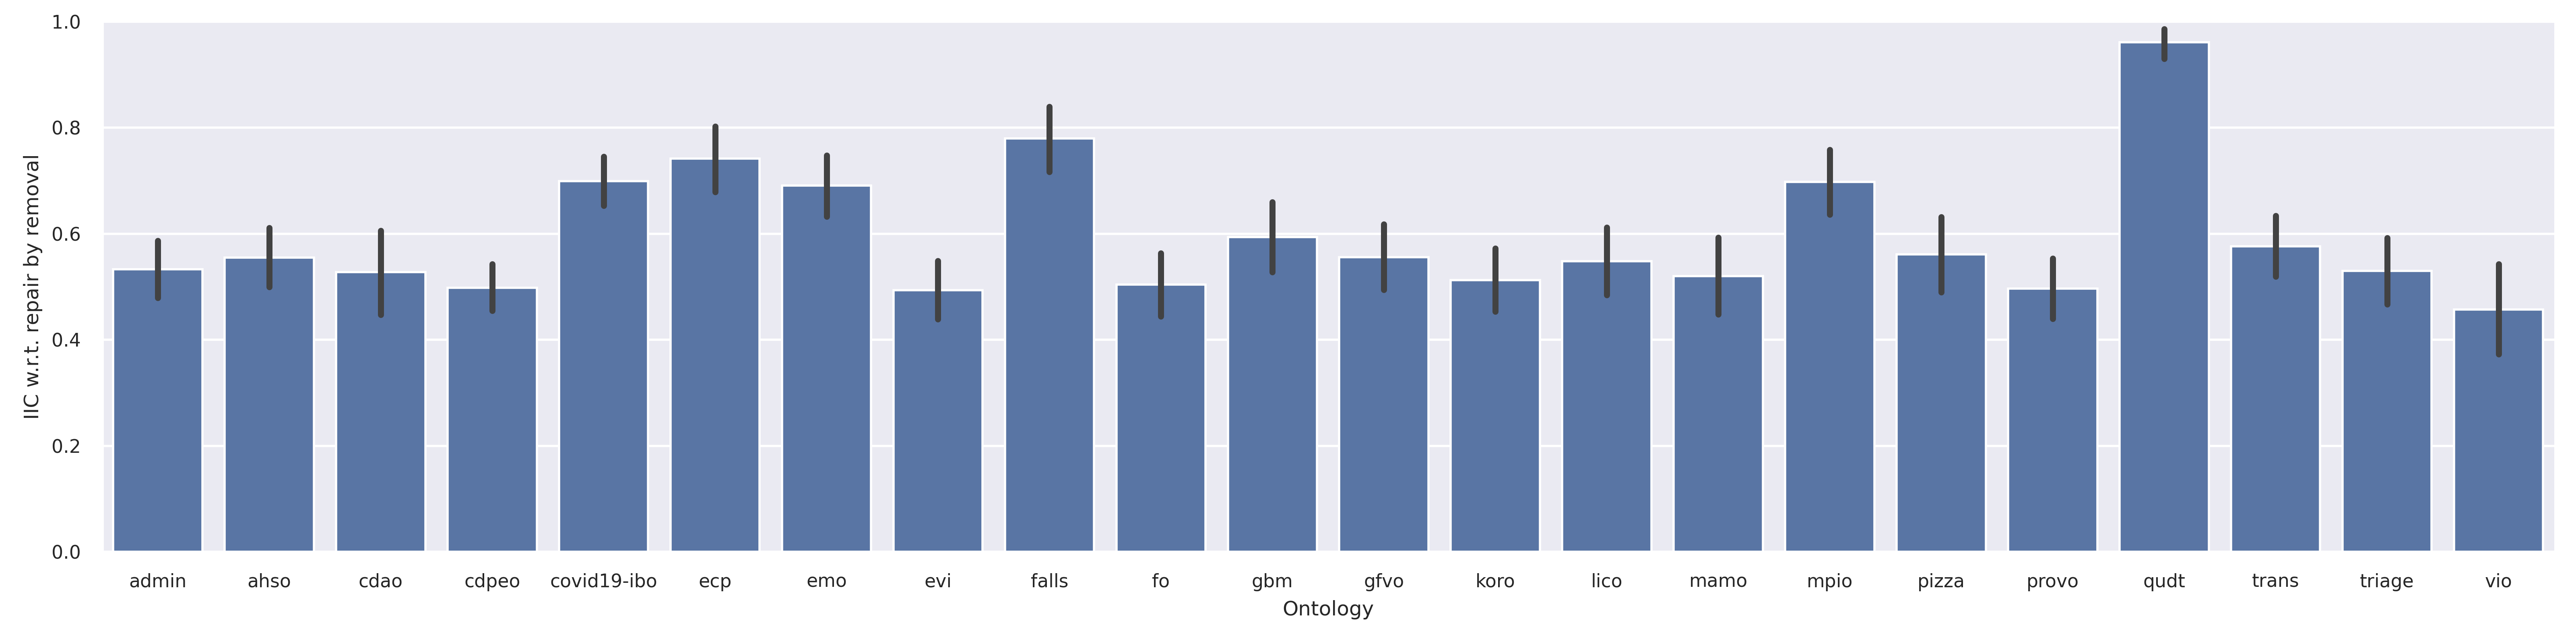
\includegraphics[width=\textwidth]{resources/iic-remove-ontology-bar.png}
  \caption{Mean IIC with respect to repair via removal per ontology. The error bars show the 95\% confidence interval.}
  \label{fig:results-remove}
\end{figure}

The results of the evaluation suggest that the repair by weakening is on average about as good or better than the repair by removal of axioms. While this supports the conclusion in \cite{troquard2018repairing} that weakening is able to retain more information than removal, the observed advantage was worse than what has been observed in \cite{troquard2018repairing}.

\begin{figure}[ht]
  \centering
  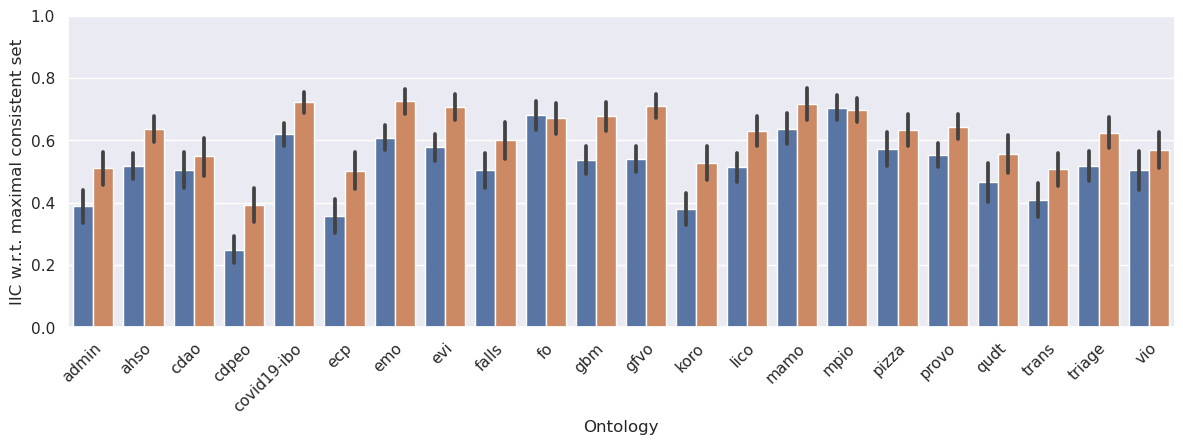
\includegraphics[width=\textwidth]{resources/iic-both-mcs-ontology-bar.png}
  \caption{Mean IIC with respect to a random maximal consistent subset. The error bars show the 95\% confidence interval. The orange bars used a variation of the repair by weakening, where axioms in the reference ontology are never weakened.}
  \label{fig:results-mcs}
\end{figure}

In contrast, it can be seen that the repair using weakening is not, in general, better than choosing a random maximal consistent subset. There are ontologies for which the repair by weakening is on average significantly worse when comparing using IIC. This is, however, a somewhat unequal comparison. We have seen in \cref{ex:alc-weakening} also a situation in which weakening performs worse when it comes to preserving information compared to choosing a maximally consistent subset. A more equal comparison, yet still not perfect since the maximal consistent subset for the reference ontology is not chosen uniformly at random, would be to a repair algorithm that starts with the reference ontology and uses weakening to add more information from the remaining axioms. This has been implemented and evaluated, and the results can be seen as the orange bars in \cref{fig:results-mcs}. Still, this result suggests that the heuristic used for selecting bad axioms is not reliable for preserving information, at least when measured using IIC. It has not been closely studied what causes the repair by weakening to significantly lose for some ontologies while being clearly preferred in others. Interestingly, there are also some cases in which the weakening based repair performs better against a random maximal consistent subset than against the repair by removal.

To overcome some weaknesses of the IIC, especially that it does not account for subsumptions between roles or complex concept expressions, tests were also carried out using an extended version of the inferred class hierarchy and IIC, adding to it subsumptions between subconcepts and roles.

\begin{definition}
  The \emph{extended inferred class hierarchy} of an ontology $\Omc$ is given by
  \begin{align*}
    \Inf^+(\Omc) ={} & \{ C \sqsubseteq D \mid C, D \in \sub(\Omc) \text{ and } C \sqsubseteq_\Omc D \} \\
    & \cup \{ R \sqsubseteq S \mid R, S \in \Lmc(N_R) \text{ and } R \sqsubseteq_\Omc S \} \enspace.
  \end{align*}
  The \emph{extended inferable information content} (IIC$^+$) of an ontology $\Omc_1$ with respect to another ontology $\Omc_2$ is given by
  \begin{align*}
    \qual^+(\Omc_1, \Omc_2) = \frac{| \Inf^+(\Omc_1) \setminus \Inf^+(\Omc_2) |}{|\Inf^+(\Omc_1) \setminus \Inf^+(\Omc_2)| + |\Inf^+(\Omc_2) \setminus \Inf^+(\Omc_1)|} \enspace,
  \end{align*}
\end{definition}

Of course, this new measure still only captures a small part of all consequences, but it should provide more accurate results when it comes to information about subconcepts and roles. When evaluating the experiment outcomes, we see that the values produced by IIC and IIC$^+$ are very similar. As may be expected, the repair by weakening is preferred slightly more strongly when using IIC$^+$. \Cref{fig:results-eiic} shows the comparison between IIC and IIC$^+$ for repair using axiom weakening w.r.t. repair by removal. The differences between IIC and IIC$^+$ are somewhat stronger when comparing against the repair using a random maximal consistent subset, but the differences are still not particularly noteworthy.

\begin{figure}[ht]
  \centering
  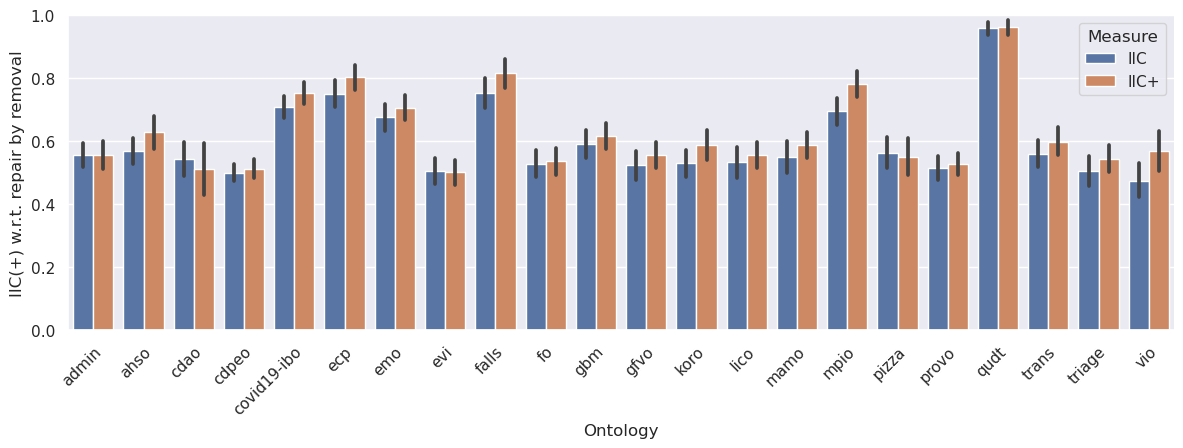
\includegraphics[width=\textwidth]{resources/iic-eiic-ontology-bar.png}
  \caption{Mean IIC and IIC$^+$ with respect to repair by removal per ontology. The error bars show the 95\% confidence interval.}
  \label{fig:results-eiic}
\end{figure}


\section{Effectiveness of Caching in Cover Computation}


As discussed in \cref{cache-impl}, to accelerate the computation of upward and downward covers, a cache was added to avoid repeated calls to the reasoner when the necessary information can already be inferred from previous computations. This section will discuss the experiments performed to evaluate the effectiveness of this cache.

Three versions of the upward and downward cover have been considered, the uncached version that calls the reasoner for every subsumption query, a version that caches only the exact queries that were already made previously, and finally the version that additionally infers some additional information from the transitivity of subsumption as listed in \cref{algo:cached-subs}. The experiment uses some of the same ontologies as have been used for the previously discussed evaluation of the repair quality. From the logical axioms of each ontology were selected, uniformly at random, one hundred groups with a fixed number of axioms. The same axioms may be selected multiple times. Each of the groups was then tested with a separate instance of the cache. The rationale behind testing with different group sizes is that the cache will obviously have a greater impact when the same cache can be reused for more cover computations. In each test run, the axiom weakening operator was applied to each axiom and the number of reasoner calls and (real) time taken were measured. The weakening operator used the complete (after preprocessing) ontology as the reference ontology. The test has further been performed using different OWL 2 DL reasoners. The final results of the evaluation can be seen in \cref{table:results-cache-calls} and are visualized in \cref{fig:results-cache-calls} and \cref{fig:results-cache-time}. Note that a logarithmic y-axis has been used for both plots.

\begin{table}[ht]
  \scriptsize
  \centering
  \begin{tabular}{|l|rrr|rrr|rrr|}
    \cline{2-10}
    \multicolumn{1}{l|}{} & \multicolumn{9}{c|}{\hspace{-4mm}Reasoner calls per weakening} \\
    \multicolumn{1}{l|}{} & \multicolumn{3}{c}{Full caching} & \multicolumn{3}{c}{Simple caching} & \multicolumn{3}{c|}{No caching} \\
    \multicolumn{1}{l|}{} & \multicolumn{1}{c}{1} & \multicolumn{1}{c}{10} & \multicolumn{1}{c}{100} & \multicolumn{1}{c}{1} & \multicolumn{1}{c}{10} & \multicolumn{1}{c}{100} & \multicolumn{1}{c}{1} & \multicolumn{1}{c}{10} & 100 \\
    \hline
    admin & 1096 & 222 & 35
      & 15138 & 2115 & 236
      & 41105 & 41288 & 41751 \\
    cdpeo & 2110 & 522 & 75
      & 13621 & 2694 & 312
      & 29051 & 28617 & 29315 \\
    emo & 2652 & 1355 & 258
      & 7781 & 2784 & 619
      & 12524 & 12134 & 12552 \\
    gbm & 3019 & 1074 & 168
      & 12572 & 3284 & 503
      & 19490 & 21330 & 20801 \\
    gfvo & 1737 & 575 & 80
      & 2828 & 1524 & 293
      & 4058 & 4104 & 4003 \\
    koro & 2006 & 591 & 80
      & 5154 & 2272 & 382
      & 7271 & 7181 & 7422 \\
    mamo &  1984 & 511 & 61
      & 3557 & 1488 & 234
      & 5060 & 5059 & 4998 \\
    \hline
    Overall & 2086 & 693 & 108
      & 8664 & 2309 & 368
      & 16937 & 17102 & 17263 \\
    \hline
  \end{tabular}
  \caption{Results of the evaluation of cache effectiveness. The mean number of reasoner calls required for a single application of the axiom weakening operator on randomly selected axioms of the ontology is given for different degrees of cache reuse. The cache is reused of one, ten, or one hundred successive operator applications.}
  \label{table:results-cache-calls}
\end{table}

\begin{figure}[ht]
  \centering
  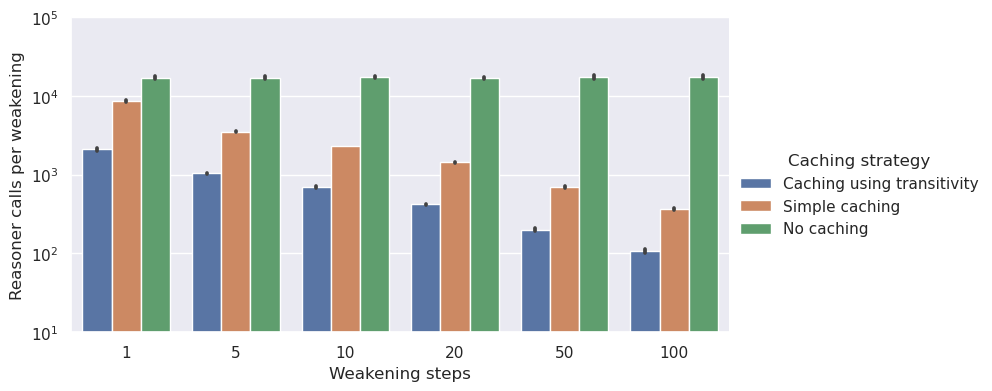
\includegraphics[width=\textwidth]{resources/calls-cache-bar.png}
  \caption{The mean number of reasoner calls needed for a single application of the axiom weakening operator, averaged over the tested ontologies.}
  \label{fig:results-cache-calls}
\end{figure}

\begin{figure}[ht]
  \centering
  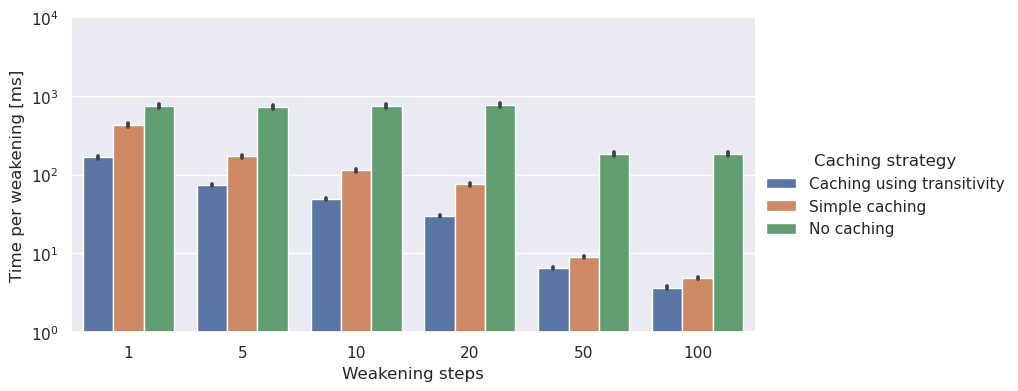
\includegraphics[width=\textwidth]{resources/time-cache-bar.png}
  \caption{Average time required per application of the axiom weakening operator with different caching strategies. The results are averaged over the tested ontologies and the reasoners FaCT++, JFact, Openllet, and HermiT.}
  \label{fig:results-cache-time}
\end{figure}

We can see clearly from the results that the cache is indeed effective at lowering both the number of reasoner calls and execution time. The simple caching method alone provides a dramatic decrease in the number of reasoner calls, especially at higher group sizes. The algorithm that can additionally exploit the transitivity of the relation performs even better, also with a smaller number of weakening steps. The difference when looking at the execution time is significantly smaller. This can likely be attributed largely to internal caching performed by the reasoners. This would also explain the observed variation when it comes to the relative improvement between different reasoners. It can be concluded that the addition of the cache greatly benefits the computation of the axiom weakening operator, especially if it can be reused for many applications of the same weakening operator.



\section{Evaluating Required Execution Time}


The performance of the axiom weakening based repair algorithm shown in \cref{algo:repair-weaken} has also been evaluated. During each repair via axiom weakening, the time taken and the number of calls to the reasoner have been registered. Additionally, the number of steps taken by the repair using axiom weakening has been observed. Also, as mentioned in \cref{eval-quality}, the repair program was put under a timeout to prevent cases where the reasoning becomes unreasonably slow. The generation of inconsistent ontologies used a similar timeout, and the same procedure was used for situations in which the reasoner ran out of memory. Timeout of the weakening procedure are shown separately from those latter cases in the results. The frequency of these cases is indicated as percentage of the overall runs finished vs started. The results of this evaluation are presented in \cref{table:results-perf} and \cref{fig:results-perf-time}.

\begin{table}[ht]
  \scriptsize
  \centering
  \begin{tabular}{|l|r@{ }lr@{ }lr@{ }lr@{ }r|}
    \cline{2-9}
    \multicolumn{1}{l|}{} & \multicolumn{2}{c}{Steps} & \multicolumn{2}{c}{Calls} & \multicolumn{2}{c}{Time [ms]} & \multicolumn{2}{c|}{Failed} \\
    \hline
    admin & 6.3 & [4.0, 9.2] & 7621 & [5601, 10118] & 9638 & [5433, 14909] & 2\% & (2\%) \\
    ahso & 2.1 & [1.7, 2.5] & 4648 & [4228, 5131] & 11469 & [8122, 15336] & 11\% & (26\%) \\
    cdao & 2.1 & [1.8, 2.5] & 16137 & [14576, 17740] & 20767 & [15204, 27269] & 19\% & (48\%) \\
    cdpeo & 1.5 & [1.3, 1.7] & 4476 & [4250, 4716] & 2050 & [1942, 2169] & 0\% & (0\%) \\
    covid19-ibo & 1.3 & [1.2, 1.5] & 14822 & [14321, 15320] & 2208 & [2126, 2296] & 4\% & (13\%) \\
    ecp & 1.3 & [1.2, 1.5] & 2020 & [1916, 2133] & 4453 & [2738, 6939] & 1\% & (14\%) \\
    emo & 1.4 & [1.3, 1.6] & 18549 & [17473, 19615] & 6582 & [4439, 9688] & 1\% & (4\%) \\
    evi & 5.0 & [3.9, 6.4] & 5955 & [4680, 7425] & 4719 & [3408, 6349] & 19\% & (64\%) \\
    falls & 1.5 & [1.3, 1.6] & 1242 & [1161, 1331] & 874 & [843, 909] & 1\% & (5\%) \\
    fo & 1.6 & [1.4, 1.8] & 1295 & [1179, 1423] & 1090 & [1025, 1164] & 38\% & (61\%) \\
    gbm & 1.5 & [1.3, 1.6] & 7608 & [7070, 8131] & 2954 & [2808, 3117] & 0\% & (0\%) \\
    gfvo & 1.8 & [1.6, 2.0] & 4167 & [3864, 4501] & 2404 & [2258, 2569] & 0\% & (0\%) \\
    koro & 1.9 & [1.7, 2.2] & 6195 & [5697, 6706] & 2456 & [2277, 2648] & 0\% & (0\%) \\
    lico & 2.6 & [2.2, 2.9] & 6638 & [6105, 7186] & 3709 & [3400, 4077] & 1\% & (22\%) \\
    mamo & 2.5 & [2.2, 2.9] & 4667 & [4228, 5128] & 2215 & [2046, 2403] & 0\% & (0\%) \\
    mpio & 2.2 & [1.8, 2.6] & 1908 & [1720, 2133] & 987 & [913, 1078] & 9\% & (30\%) \\
    pizza & 2.0 & [1.7, 2.3] & 7550 & [6723, 8419] & 26767 & [20554, 34014] & 28\% & (55\%) \\
    provo & 4.9 & [3.7, 6.3] & 6851 & [5383, 8465] & 8878 & [5962, 12348] & 4\% & (8\%) \\
    qudt & 1.1 & [1.0, 1.2] & 7044 & [6816, 7291] & 6658 & [4229, 9672] & 9\% & (38\%) \\
    trans & 3.2 & [1.8, 5.1] & 4384 & [3213, 5894] & 3684 & [1610, 6513] & 0\% & (5\%) \\
    triage & 3.2 & [2.4, 4.3] & 5166 & [4255, 6351] & 8979 & [6084, 13102] & 28\% & (51\%) \\
    vio & 2.5 & [2.1, 3.0] & 9476 & [8628, 10327] & 15199 & [10496, 20803] & 3\% & (7\%) \\
    \hline
  \end{tabular}
  \caption{Results of the evaluation with respect to performance. Number of weakening iterations, reasoner calls, and total repair time are given as sample mean, with 95\% confidence interval in brackets. The frequency of failed runs is shown as percentage of repairs by weakening that were started but not completed. In parentheses, the percentage of total failed runs, including those with timeout during generation of the inconsistent ontology. Attempts that failed were not considered for the other values.}
  \label{table:results-perf}
\end{table}

\begin{figure}[ht]
  \centering
  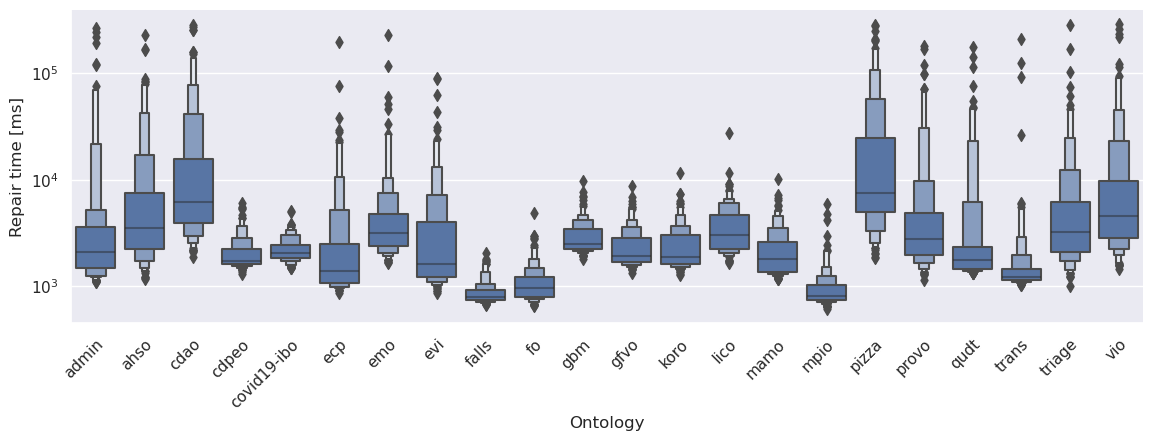
\includegraphics[width=\textwidth]{resources/time-ontology-violin.png}
  \caption{Distribution of (real) execution time required for repairing a single ontology using axiom weakening. The two darkest blue boxes represent (together) half of the samples, with the line in the middle indicating the median. Each lighter box represents half the samples of the boxes one step darker, and all remaining outliers are marked. Attempts that failed by timeout or other errors were not considered.}
  \label{fig:results-perf-time}
\end{figure}

As is visible from the results, the number of reasoner calls and the execution time can vary significantly. The execution times were generally reasonable when a run was able to complete within the time limit, with most of them completing within 2 minutes, even though the time limit was set to 5 minutes. A significant number of runs, however, were affected by the timeout or other errors. It has not been looked deeper into what causes these issues.




\chapter{Conclusion and Future Work} \label{conclusion}


This thesis has proposed refinement operators and an axiom weakening operator for all aspects of \SROIQ and shown that for repairs of inconsistent ontologies weakening can, in some cases, significantly outperform removal. The proposed approaches have been implemented both for performing the empirical evaluation and in a Protégé plugin that allows users to use the techniques described in this thesis, both for manually weakening axioms and for automatically repairing ontologies. Some ideas implemented for and discussed in the thesis, like the repair approaches focusing on finding better repairs discussed in \cref{best-repair-impl} or the relaxed RIA weakening mentioned in \cref{rbox-alternative}, have not yet been fully studied and still have to be evaluated.

Better ways for users to interact with and guide the repair process may also be studied. It can also be seen that the repair algorithm likely needs better heuristics to steer the selection of bad and weakened axioms in order to result in better repairs. This may involve also the use of domain specific information and heuristics that could steer the repair process to choose repairs that make sense also from a modelling perspective. The termination of the proposed repair algorithm should be studied, as has been done in \cite{confalonieri2020towards}. Further additions to the refinement operators may also be studied in more detail, e.g., using non-simple roles in the upward and downward covers in certain contexts. Relaxing the allowed weakening for RIAs may also be considered, and to cover also extensions to regularity conditions such as those studied in \cite{DBLP:conf/cade/Kazakov10}. Future work could further focus on finding robust measures for comparing the quality of repairs. Different applications for the axiom weakening and refinement operators, like the ones studied for concept combination in \cite{righetti2022asymmetric}, are now also able to be explored using more expressive DLs.



\printbibliography

\appendix

\chapter{Closure over RBox Weakening} \label{proof-weakening}

\begin{lemma} \label{lem:subseteq-up}
For all $r' \in \mathrm{UpCover}_\mathcal{O}(r)$ and every model $M$ of $\mathcal{O}$, $r^M \subseteq r'^M$.
\end{lemma}

\begin{proof}
Following the definition of $\mathrm{UpCover}_\mathcal{O}(\cdot)$, $r \sqsubseteq_\mathcal{O} r'$ holds and by definition $r^M \subseteq r'^M$ must therefore be true in every model.
\end{proof}

\begin{lemma} \label{lem:subseteq-down}
For all $r' \in \mathrm{DownCover}_\mathcal{O}(r)$ and every model $M$ of $\mathcal{O}$, $r'^M \subseteq r^M$.
\end{lemma}

\begin{proof}
Following the definition of $\mathrm{DownCover}_\mathcal{O}(\cdot)$, $r' \sqsubseteq_\mathcal{O} r$ holds and by definition $r'^M \subseteq r^M$ must therefore be true in every model.
\end{proof}

\begin{lemma} \label{lem:entailed-right}
The RBox $\mathcal{R}'$, obtained by replacing any RIA $\phi = s_1 \circ \cdots \circ s_n \sqsubseteq r$ in the regular RBox $\mathcal{R}$ with a RIA $\phi' = s_1 \circ \cdots \circ s_n \sqsubseteq r'$ where $r \sqsubseteq_\mathcal{O} r'$, is entailed by $\mathcal{R}$.
\end{lemma}

\begin{proof}
Take an arbitrary model $M$ of $\mathcal{R}$.
All axioms in $\mathcal{R}'$ that are also in $\mathcal{R}$ are satisfied by $M$ because $M$ satisfies all axioms in $\mathcal{R}$.
We know that $r^M \subseteq r'^M$.
Since $M$ satisfies all axioms in $\mathcal{R}$, it satisfies $\phi$ meaning $s_1^M \circ \cdots \circ s_n^M \subseteq r^M$.
Using the transitivity of the subset relation on sets, we obtain $s_1^M \circ \cdots \circ s_n^M \subseteq r'^M$.
By definition, it follows that $M$ satisfies $\phi'$.
Since all other axioms of $\mathcal{R}'$ are also in $\mathcal{R}$, $M$ satisfies all axioms of $\mathcal{R}'$ and is therefore a model for $\mathcal{R}'$.
\end{proof}

\begin{lemma} \label{lem:entailed-left}
The RBox $\mathcal{R}'$, obtained by replacing any RIA $\phi = s_1 \circ \cdots \circ s_i' \circ \cdots \circ s_n \sqsubseteq r$ in the regular RBox $\mathcal{R}$ with a RIA $\phi' = s_1 \circ \cdots \circ s_i' \circ \cdots \circ s_n \sqsubseteq r$ where $s_i' \sqsubseteq_\mathcal{O} s_i$, is entailed by $\mathcal{R}$.
\end{lemma}

\begin{proof}
Take an arbitrary model $M$ of $\mathcal{R}$.
All axioms in $\mathcal{R}'$ that are also in $\mathcal{R}$ are satisfied by $M$ because $M$ satisfies all axioms in $\mathcal{R}$.
We know that $s_i'^M \subseteq s_i^M$.
Since $M$ satisfies all axioms in $\mathcal{R}$, it satisfies $\phi$ meaning $s_1^M \circ \cdots \circ s_i^M \circ \cdots \circ s_n^M \subseteq r^M$.
From $s_i'^M \subseteq s_i^M$ it follows that $s_1^M \circ \cdots \circ s_i'^M \circ \cdots \circ s_n^M \subseteq s_1^M \circ \cdots \circ s_i^M \circ \cdots \circ s_n^M$.
Using transitivity of the subset relation on sets, we obtain $s_1^M \circ \cdots \circ s_i'^M \circ \cdots \circ s_n^M \subseteq r^M$.
By definition, it follows that $M$ satisfies $\phi'$.
Since all other axioms of $\mathcal{R}'$ are also in $\mathcal{R}$, $M$ satisfies all axioms of $\mathcal{R}'$ and is therefore a model for $\mathcal{R}'$.
\end{proof}

\begin{lemma} \label{lem:entailed-dis}
The RBox $\mathcal{R}'$, obtained by replacing any role assertion $\phi = \mathrm{Dis}(s_1, s_2)$ in the regular RBox $\mathcal{R}$ with a RIA $\phi' = \mathrm{Dis}(s_1', s_2')$ where $s_1' \sqsubseteq_\mathcal{O} s_1$ and $s_2' \sqsubseteq_\mathcal{O} s_2$, is entailed by $\mathcal{R}$.
\end{lemma}

\begin{proof}
Take an arbitrary model $M$ of $\mathcal{R}$.
All axioms in $\mathcal{R}'$ that are also in $\mathcal{R}$ are satisfied by $M$ because $M$ satisfies all axioms in $\mathcal{R}$.
We know that $s_1'^M \subseteq s_1^M$ and $s_2'^M \subseteq s_2^M$.
Since $M$ satisfies all axioms in $\mathcal{R}$, it satisfies $\phi$ meaning $s_1^M \cap s_2^M = \empty$.
We know that $s_1'^M \cap s_2'^M \subseteq s_1^M \cap s_2^M = \empty$.
By definition, it follows that $M$ satisfies $\phi'$.
Since all other axioms of $\mathcal{R}'$ are also in $\mathcal{R}$, $M$ satisfies all axioms of $\mathcal{R}'$ and is therefore a model for $\mathcal{R}'$.
\end{proof}

\begin{lemma} \label{lem:regular-right}
The RBox $\mathcal{R}'$, obtained by replacing any simple RIA $\phi = s \sqsubseteq r$ in the regular RBox $\mathcal{R}$ for which $s$ is simple with a RIA $\phi' = s \sqsubseteq r'$ where $r' \in \mathbf{R}$, is regular.
\end{lemma}

\begin{proof}
Since $\mathcal{R}$ is regular, there exist a relation $\prec$ that satisfies the necessary conditions.
All axioms in $\mathcal{R}'$ that are also in $\mathcal{R}$ are $\prec$-regular.
It follows that since $s$ is simple, the new RIA is $\prec$-regular.
Since $\mathcal{R}'$ contains no other axioms, all axioms in $\mathcal{R}'$ are $\prec$-regular.
$\mathcal{R}'$ is regular since $\prec$ is an admissible regular order.
\end{proof}

\begin{lemma} \label{lem:regular-left}
The RBox $\mathcal{R}'$, obtained by replacing any RIA $\phi = s_1 \circ \cdots \circ s' \circ \cdots \circ s_n \sqsubseteq r$ in the regular RBox $\mathcal{R}$ with a RIA $\phi' = s_1 \circ \cdots \circ s' \circ \cdots \circ s_n \sqsubseteq r$ where $s'$ is simple, is regular.
\end{lemma}

\begin{proof}
Since $\mathcal{R}$ is regular, there exist a relation $\prec$ that satisfies the necessary conditions.
All axioms in $\mathcal{R}'$ that are also in $\mathcal{R}$ are $\prec$-regular.
We handle each case of $\phi$ separately:
\begin{enumerate}[label=(\roman*)]
    \item $\phi = r \circ r \sqsubseteq r$: $r \circ s' \sqsubseteq r$ ($s' \circ r \sqsubseteq r$) is $\prec$-regular because the first (last) roles in the left-hand side are equal to the right-hand side and $s'$ is simple.
    \item $\phi = \mathrm{Inv}(r) \sqsubseteq r$: $s' \sqsubseteq r$ is $\prec$-regular because $s'$ is simple.
    \item $\phi = r \circ s_1 \circ \cdots \circ s \circ \cdots \circ s_n \sqsubseteq r$ ($\phi = s_1 \circ \cdots \circ s \circ \cdots \circ s_n \circ r \sqsubseteq r$): $r \circ s_1 \circ \cdots \circ s' \circ \cdots \circ s_n \sqsubseteq r$ ($s_1 \circ \cdots \circ s' \circ \cdots \circ s_n \circ r \sqsubseteq r$) is $\prec$-regular because since the original axiom is $\prec$-regular, we know that $s_i$ is simple or $s_i \prec r$ for all $i = 1, \dots, n$. Additionally, the first (last) role on the left-hand side is equal to the right-hand side and $s'$ is simple.
    \item $\phi = s_1 \circ \cdots \circ s \circ \cdots \circ s_n \sqsubseteq r$: $s_1 \circ \cdots \circ s' \circ \cdots \circ s_n \sqsubseteq r$ is $\prec$-regular because $s'$ is simple and since the original axiom is $\prec$-regular, we know that $s_i$ is simple or $s_i \prec r$ for all $i = 1, \dots, n$.
\end{enumerate}

We conclude that the new axiom is $\prec$-regular.
Since $\mathcal{R}'$ contains no other axioms, all axioms in $\mathcal{R}'$ are $\prec$-regular.
$\mathcal{R}'$ is regular since $\prec$ is an admissible regular order.
\end{proof}

\begin{lemma} \label{lem:simple-right}
The RBox $\mathcal{R}'$ is obtained by replacing any simple RIA $\phi = s \sqsubseteq r$ in the regular RBox $\mathcal{R}$ for which $s$ is simple with a RIA $\phi' = s \sqsubseteq r'$ where $r' \in \mathbf{R}$. All roles that are simple in $\mathcal{R}$ are also simple in $\mathcal{R}'$.
\end{lemma}

\begin{proof}
Let $t$ be an arbitrary role that is simple in $\mathcal{R}$.
$t$ is simple in $\mathcal{R}'$ because:
\begin{enumerate}[label=(\roman*)]
    \item  $t \not= u$, otherwise $t$ would not be simple in $\mathcal{R}$.
    \item $t$ does not appear on the right-hand side of a complex RIA. The only new axiom in $\mathcal{R}'$ is $\phi'$.  $\phi'$ is a simple RIA.
    \item $t$ does not appear in a simple RIA where the left-hand side is non-simple. The only new axiom in $\mathcal{R}'$ is $\phi'$. The left-hand side of $\phi'$, $s$, is simple.
    \item $\mathrm{Inv}(t)$ is simple because it is simple in $\mathcal{R}$ and the above three points hold also for $\mathrm{Inv}(t)$.
\end{enumerate}

Since $t$ is an arbitrary simple role from $\mathcal{R}$, all simple roles in $\mathcal{R}$ are simple in $\mathcal{R}'$.
\end{proof}

\begin{lemma} \label{lem:simple-left}
The RBox $\mathcal{R}'$ is obtained by replacing any RIA $\phi = s_1 \circ \cdots \circ s' \circ \cdots \circ s_n \sqsubseteq r$ in the regular RBox $\mathcal{R}$ with a RIA $\phi' = s_1 \circ \cdots \circ s' \circ \cdots \circ s_n \sqsubseteq r$ where $s'$ is simple. All roles that are simple in $\mathcal{R}$ are also simple in $\mathcal{R}'$.
\end{lemma}

\begin{proof}
Let $t$ be an arbitrary role that is simple in $\mathcal{R}$.
$t$ is simple in $\mathcal{R}'$ because:
\begin{enumerate}
    \item  $t \not= u$, otherwise $t$ would not be simple in $\mathcal{R}$.
    \item $t$ does not appear on the right-hand side of a complex RIA. The only new axiom in $\mathcal{R}'$ is $\phi'$. If $\phi'$ is a complex RIA and $t = r$, then $t$ would not be simple in $\mathcal{R}$ because it is on the right-hand side of the complex RIA $\phi$. This contradicts our assumption that $t$ is simple.
    \item $t$ does not appear in a simple RIA where the left-hand side is non-simple. The only new axiom in $\mathcal{R}'$ is $\phi'$. The left-hand side of $\phi'$, $s'$, is simple.
    \item $\mathrm{Inv}(t)$ is simple because it is simple in $\mathcal{R}$ and the above three points hold also for $\mathrm{Inv}(t)$.
\end{enumerate}

Since $t$ is an arbitrary simple role from $\mathcal{R}$, all simple roles in $\mathcal{R}$ are simple in $\mathcal{R}'$.
\end{proof}

\begin{theorem} \label{the:closed}
The set of well-formed $\mathcal{SROIQ}$ ontologies is closed under axiom weakening. That is, given a valid $\mathcal{SROIQ}$ ontology $\mathcal{O}$ with a regular RBox $\mathcal{R}$, the ontology $\mathcal{O}' = \mathcal{O} \setminus \{\alpha\} \cup \{\alpha'\}$ obtained by replacing any axiom $\alpha \in \mathcal{O}$ with a weakening $\alpha' \in g_\mathcal{O}(\alpha)$ is also a valid $\mathcal{SROIQ}$ ontology.
\end{theorem}

\begin{proof}
We must show that the axioms resulting from weakening are syntactically correct, that no non-simple role is used in disjoint role axioms, cardinality restrictions, or self restrictions, and that the resulting RBox is regular.

Regularity of the RBox follows from \cref{lem:regular-right} and \cref{lem:regular-left}, since those are the only types of transformations performed on the RIAs, and regularity depends only on the RIAs. Similarly, it follows  from \cref{lem:simple-right} and \cref{lem:simple-left} that all roles simple in $\mathcal{O}$ are also simple in $\mathcal{O}'$. This means all cardinality or self restriction for which the role is not changed, still use a simple role.

Numbers and roles in the axioms are replaced, if at all, always with either a number or role respectively. This is ensured by the definition of the upward and downward cover. The covers return only non-negative numbers, roles that appear in the signature of the ontology, or the inverse of those roles. Since all roles returned by the upward and downward covers are simple in $\mathcal{O}$ and therefore still simple in $\mathcal{O}'$, it is not possible to replace a simple role with a non-simple role in a disjoint role axiom.

Concepts are replaced always with another valid concept, since the refinement operator, given a well-formed concept, returns only well-formed concept expressions.
By induction, the refinement operator returns either:

\begin{enumerate}[label=(\roman*)]
    \item The result of the upward or downward covers. These are by definition subconcepts of the original ontology, which, since it appears in the original ontology, must be well-formed.
    \item An expression in which one part of the input is replaced:
        \begin{itemize}
            \item A number or role is replaced with a role from the upward or downward cover. As mentioned above, the covers return only respectively valid numbers or roles. Since all roles returned are simple in $\mathcal{O}'$ it is not possible that a non-simple role is used in a cardinality or self restriction.
            \item A concept is replaced with the output of applying the refinement operator to the concept, that it replaces. Since the concept that is replaced is in the original ontology, it is well-formed, and the replacement is a well-formed concept expression given our inductive hypothesis.
        \end{itemize}
\end{enumerate}
\end{proof}


\chapter{Axiom Weakening in OWL 2 DL} \label{weakening-owl-2-dl}

Since OWL 2 DL is reducible to $\mathcal{SROIQ}$ it would be sufficient to perform this normalization and then apply the weakening as described to the resulting $\mathcal{SROIQ}$ ontology. This transformation is unproblematic in some contexts, for example if the result is only going to be used for automatic reasoning tasks. However, if the output must be further manipulated by a user of the system, the added noise introduced by the normalization may cause confuting and hinder understanding. Further, weakening OWL 2 DL ontologies directly can be seen as a heuristic, giving an indication as to which weakening might make sense from a modelling perspective.

\begin{example}
OWL has an axiom $\mathrm{DisjointClasses}(C_1, \dots, C_n)$\footnote{In the rest of this section, the OWL 2 functional syntax (cf. \cite{motik2009owl_spec}) will be used.} that allows specifying that a set of classes all are pairwise disjoint. $C_i \sqcap C_j \sqsubseteq \bot$ for all $i \not= j = 1, \dots, n$. One reasonable approach to weakening the OWL axiom is to replace any of the classes $C_i$ with a more specific class $C_i' \in \rho_\mathcal{O}(C_i)$. In contrast, after normalization, there will be $n - 1$ occurrences of $C_i$. It is unlikely, increasingly so with growing $n$, that all such occurrences will be weakened to the same concept. After weakening the normalized ontology, it is thus in general not possible to reconstruct the disjointness axiom.
\end{example}

It should be noted that working directly with OWL 2 axioms will make repairs less gentle. For some axiom types, it is not obvious how they could reasonably be weakened to another single axiom. For these kinds of axioms, removal is the only available weakening.

\begin{example}
The OWL axiom $\mathrm{EquivalentClasses}(C_1, \dots, C_n)$ can not easily be weakened. One option for weakening is removing one of the arguments. The axiom would be normalized to a set of $\mathrm{SubClassOf}$ axioms, for which both the subclass and superclasses can be modified. It is evident that this is more gentle than completely removing arguments.
\end{example}

For OWL 2 DL we must follow the same restrictions, when it comes to regularity and simplicity of roles, as for $\mathcal{SROIQ}$. The same definitions for the upward and downward covers, $\mathrm{UpCover}_\mathcal{O}$ and $\mathrm{DownCover}_\mathcal{O}$, are used. We define the refinement operator $\zeta_{\uparrow,\downarrow}$ for OWL 2 DL as follows:

\begingroup
\scriptsize
\begin{align*}
    \zeta_{\uparrow, \downarrow}(A) = \;& \uparrow (A) \qquad \text{for } A \in \mathrm{N}_c \cup \mathbf{R} \cup \{ \top , \bot \} \\
    \zeta_{\uparrow, \downarrow}(\mathrm{ObjectComplementOf}(C)) = \;& \uparrow (\mathrm{ObjectComplementOf}(C)) \\& \cup \{ \mathrm{ObjectComplementOf}(C')  \mid C' \in \zeta_{\downarrow, \uparrow} (C) \} \\
    \zeta_{\uparrow, \downarrow}(\mathrm{ObjectIntersectionOf}(C_1, \dots, C_n)) = \;& \uparrow (\mathrm{ObjectIntersectionOf}(C_1, \dots, C_n)) \\& \cup \bigcup_{i=1}^n \{\mathrm{ObjectIntersectionOf}(C_1, \dots, C_i', \dots C_n)  \mid C_i' \in \zeta_{\uparrow, \downarrow} (C_i) \} \\
    \zeta_{\uparrow, \downarrow}(\mathrm{ObjectUnionOf}(C_1, \dots, C_n)) = \;& \uparrow (\mathrm{ObjectUnionOf}(C_1, \dots, C_n)) \\& \cup \bigcup_{i=1}^n  \{ \mathrm{ObjectUnionOf}(C_1, \dots, C_i', \dots C_n)  \mid C_i' \in \zeta_{\uparrow, \downarrow} (C_i)\} \\
    \zeta_{\uparrow, \downarrow}(\mathrm{ObjectAllValuesFrom}(r, C)) = \;& \uparrow (\mathrm{ObjectAllValuesFrom}(r, C)) \\& \cup \{\mathrm{ObjectAllValuesFrom}(r', C) \mid r' \in \zeta_{\downarrow, \uparrow} (r)\} \\& \cup \{\mathrm{ObjectAllValuesFrom}(r, C') \mid C' \in \zeta_{\uparrow, \downarrow}  (C)\} \\
    \zeta_{\uparrow, \downarrow}(\mathrm{ObjectSomeValuesFrom}(r, C)) = \;& \uparrow (\mathrm{ObjectSomeValuesFrom}(r, C)) \\&  \cup \{\mathrm{ObjectSomeValuesFrom}(r', C) \mid r' \in \zeta_{\uparrow, \downarrow} (r)\} \\& \cup \{\mathrm{ObjectSomeValuesFrom}(r, C') \mid C' \in \zeta_{\uparrow, \downarrow}  (C)\} \\
    \zeta_{\uparrow, \downarrow}(\mathrm{ObjectHasSelf}(r)) = \;& \uparrow (\mathrm{ObjectHasSelf}(r)) \\&  \cup \{\mathrm{ObjectHasSelf}(r') \mid r' \in \zeta_{\uparrow, \downarrow}(r)\} \\
    \zeta_{\uparrow, \downarrow}(\mathrm{ObjectHasValue}(r, a)) = \;& \uparrow (\mathrm{ObjectHasValue}(r, a)) \\&  \cup \{\mathrm{ObjectHasValue}(r', a) \mid r' \in \zeta_{\uparrow, \downarrow} (r)\} \\&  \cup \{\mathrm{ObjectSomeValuesFrom}(r, A) \mid A \in \zeta_{\uparrow, \downarrow}  (\{a\})\} \\
    \zeta_{\uparrow, \downarrow}(\mathrm{ObjectMaxCardinality}(n, r, C)) = \;& \uparrow (\mathrm{ObjectMaxCardinality}(n, r, C)) \\&  \cup \{\mathrm{ObjectMaxCardinality}(n', r, C) \mid n' \in \; \uparrow (n)\} \\&   \cup \{\mathrm{ObjectMaxCardinality}(n, r', C) \mid r' \in \zeta_{\downarrow, \uparrow}(r)\} \\&  \cup \{\mathrm{ObjectMaxCardinality}(n, r, C') \mid C' \in \zeta_{\downarrow, \uparrow} (C)\} \\
    \zeta_{\uparrow, \downarrow}(\mathrm{ObjectMinCardinality}(n, r, C)) = \;& \uparrow (\mathrm{ObjectMinCardinality}(n, r, C)) \\& \cup \{\mathrm{ObjectMinCardinality}(n', r, C) \mid n' \in \; \downarrow (n)\} \\& \cup \{\mathrm{ObjectMinCardinality}(n, r', C) \mid r' \in \zeta_{\uparrow, \downarrow}(r)\} \\& \cup \{\mathrm{ObjectMinCardinality}(n, r, C') \mid C' \in \zeta_{\uparrow, \downarrow} (C)\} \\
    \zeta_{\uparrow, \downarrow}(\mathrm{ObjectExactCardinality}(n, r, C)) = \;& \uparrow (\mathrm{ObjectExactCardinality}(n, r, C)) \\& \cup \{ \phi_1 \sqcap \phi_2   \mid \phi_1 \in \zeta_{\uparrow, \downarrow} (\mathrm{ObjectMaxCardinality}(n, r, C)) \\ \;& \qquad \land \phi_2 \in \zeta_{\uparrow, \downarrow} (\mathrm{ObjectMinCardinality}(n, r, C)) \} \\
    \zeta_{\uparrow, \downarrow}(\mathrm{ObjectOneOf}(a_1, \dots, a_n)) = \;& \uparrow (\mathrm{ObjectOneOf}(a_1, \dots, a_n))
\end{align*}
\endgroup

Using this abstract refinement operator, we build two concrete refinement operators, a generalization operator $\gamma_\mathcal{O} = \zeta_{\mathrm{UpCover}_\mathcal{O}, \mathrm{DownCover}_\mathrm{O}}$ and a specialization operator $\rho_\mathcal{O} = \zeta_{\mathrm{DownCover}_\mathcal{O}, \mathrm{UpCover}_\mathcal{O}}$. Using these generalization and specialization operators we, then define the axiom weakening operator $g_\mathcal{O}$ for OWL 2 DL axioms as follows:

\begingroup
\scriptsize
\begin{align*}
    g_\mathcal{O}(\mathrm{SubClassOf}(C, D)) =& \{\mathrm{SubClassOf}(C', D) \mid C' \in \rho_\mathcal{O} (C)\} \\& \cup \{\mathrm{SubClassOf}(C, D') \mid D' \in \gamma_\mathcal{O}  (D)\} \\
    g_\mathcal{O}(\mathrm{ClassAssertion}(C, a)) =& \{\mathrm{ClassAssertion}(C', a) \mid C' \in \gamma_\mathcal{O}  (C)\} \\
    g_\mathcal{O}(\mathrm{ObjectPropertyAssertion}(r, a)) =& \{\mathrm{ObjectPropertyAssertion}(r', a) \mid r' \in \gamma_\mathcal{O}  (r)\} \\& \cup \{ \mathrm{ObjectPropertyAssertion}(r, a), \bot \sqsubseteq \top \} \\
    g_\mathcal{O}(\mathrm{NegativeObjectPropertyAssertion}(r, a)) =& \{\mathrm{NegativeObjectPropertyAssertion}(r', a) \mid r' \in \rho_\mathcal{O}  (r)\} \\& \cup \{\mathrm{NegativeObjectPropertyAssertion}(r, a), \bot \sqsubseteq \top \} \\
    g_\mathcal{O}(\mathrm{SameIndividual}(a_1, \dots, a_n)) =& \bigcup_{i=1}^n \{ \mathrm{SameIndividual}(\{a_1, \dots, a_n\} \setminus \{a_i\}) \} \\& \cup \{ \mathrm{SameIndividual}(a_1, \dots, a_n)\} \\
    g_\mathcal{O}(\mathrm{DifferentIndividuals}(a_1, \dots, a_n)) =& \bigcup_{i=1}^n \{ \mathrm{DifferentIndividuals}(\{a_1, \dots, a_n\} \setminus \{a_i\}) \} \\& \cup \{ \mathrm{DifferentIndividuals}(a_1, \dots, a_n)\} \\
    g_\mathcal{O}(\mathrm{EquivalentClasses}(C_1, \dots, C_n)) =& \bigcup_{i=1}^n \{ \mathrm{EquivalentClasses}(\{C_1, \dots, C_n\} \setminus \{C_i\}) \} \\& \cup \{ \mathrm{EquivalentClasses}(C_1, \dots, C_n) \} \\
    g_\mathcal{O}(\mathrm{DisjointClasses}(C_1, \dots, C_n)) =& \bigcup_{i=1}^n \{ \mathrm{DisjointClasses}(C_1, \dots, C_i', \dots, C_n) \mid C_i' \in \rho_\mathcal{O}(C_i) \} \\
    g_\mathcal{O}(\mathrm{DisjointUnion}(D, C_1, \dots, C_n)) =& \{ \mathrm{DisjointUnion}(D, C_1, \dots, C_n), \bot \sqsubseteq \top \} \\
    g_\mathcal{O}(\mathrm{EquivalentObjectProperties}(r_1, \dots, r_n)) =& \bigcup_{i=1}^n \{ \mathrm{EquivalentObjectProperties}(\{r_1, \dots, r_n\} \setminus \{r_i\}) \} \\& \cup \{ \mathrm{EquivalentObjectProperties}(r_1, \dots, r_n) \} \\
    g_\mathcal{O}(\mathrm{InverseObjectProperties}(s, r)) =& \{ \mathrm{InverseObjectProperties}(s, r), \bot \sqsubseteq \top \} \\
    g_\mathcal{O}(\mathrm{FunctionalObjectProperty}(r)) =& \{ \mathrm{FunctionalObjectProperty}(r), \bot \sqsubseteq \top \} \\
    g_\mathcal{O}(\mathrm{InverseFunctionalObjectProperty}(r)) =& \{ \mathrm{InverseFunctionalObjectPro}(r), \bot \sqsubseteq \top \} \\
    g_\mathcal{O}(\mathrm{SymmetricObjectProperty}(r)) =& \{ \mathrm{SymmetricObjectProperty}(r), \bot \sqsubseteq \top \} \\
    g_\mathcal{O}(\mathrm{AsymmetricObjectProperty}(r)) =& \{ \mathrm{AsymmetricObjectProperty}(r), \bot \sqsubseteq \top \} \\
    g_\mathcal{O}(\mathrm{TransitiveObjectProperty}(r)) =& \{ \mathrm{TransitiveObjectProperty}(r), \bot \sqsubseteq \top \} \\
    g_\mathcal{O}(\mathrm{ReflexiveObjectProperty}(r)) =& \{ \mathrm{ReflexiveObjectProperty}(r), \bot \sqsubseteq \top \} \\
    g_\mathcal{O}(\mathrm{IrreflexiveObjectProperty}(r)) =& \{ \mathrm{IrreflexiveObjectProperty}(r), \bot \sqsubseteq \top \} \\
    g_\mathcal{O}(\mathrm{ObjectPropertyDomain}(r, C)) =& \{\mathrm{ObjectPropertyDomain}(r, C') \mid C' \in \gamma_\mathcal{O}  (C)\} \\
    g_\mathcal{O}(\mathrm{ObjectPropertyRange}(r, C)) =& \{\mathrm{ObjectPropertyRange}(r, C') \mid C' \in \gamma_\mathcal{O}  (C)\} \\
    g_\mathcal{O}(\mathrm{SubObjectPropertyOf}(s, r)) =& \{\mathrm{SubObjectPropertyOf}(s', r) \mid s' \in \rho_\mathcal{O} (s)\} \\& \cup \{\mathrm{SubObjectPropertyOf}(s, r') \mid r' \in \gamma_\mathcal{O}  (r) \land r \text{ is simple}\} \\& \cup \{ \bot \sqsubseteq \top \} \\
    g_\mathcal{O}(\mathrm{SubObjectPropertyOf}(\qquad \qquad \qquad \qquad &\\\mathrm{ObjectPropertyChain}(s_1, \dots, s_n), r)) =& \{\mathrm{SubObjectPropertyOf}( \\& \qquad \mathrm{ObjectPropertyChain}(s_1, \dots, s_i', \dots, s_n), r) \mid s_i' \in \rho_\mathcal{O} (s_i)\} \\& \cup \{\mathrm{SubObjectPropertyOf}( \\& \quad \qquad \mathrm{ObjectPropertyChain}(s_1, \dots, s_n), r)\} \\
    g_\mathcal{O}(\mathrm{DisjointObjectProperties}(r_1, \dots, r_n)) =& \bigcup_{i=1}^n \{ \mathrm{DisjointObjectProperties}(r_1, \dots, r_i', \dots, r_n) \mid r_i' \in \rho_\mathcal{O}(r_i) \}
\end{align*}
\endgroup


\end{document}
